\section{实验结果与分析}
\subsection{Cache仿真结果分析}
\subparagraph{仿真代码设计}
为了验证实验结果的正确性,我们采用以下代码对工程进行仿真模拟:
\begin{lstlisting}[language=Verilog]
module core_sim;
	reg clk, rst;

	RV32core core(
		.debug_en(1'b0),
		.debug_step(1'b0),
		.debug_addr(7'b0),
		.debug_data(),
		.clk(clk),
		.rst(rst),
		.interrupter(1'b0)
	);

	initial begin
	clk = 0;
	rst = 1;
	#2 rst = 0;
	end
	always #1 clk = ~clk;

endmodule 
\end{lstlisting}

测试使用的代码如下
\begin{lstlisting}[language=verilog]
| addi  x0, x0, 0  |
| lw  x2, 4(x0)    |
| lw  x4, 8(x0)    |
| add  x1, x2, x4  |
| addi  x3, x1, -1 |
| lw  x5, 12(x0)   |
| lw  x6, 16(x0)   |
| lw  x7, 20(x0)   |
| sub  x8,x4,x2    |
| addi  x9,x10,-3  |
| beq x4,x5,label0 |
| beq x4,x4,label0 |
| addi  x20,x0,48  |
| addi  x20,x0,52  |
| addi  x20,x0,56  |
| addi  x0, x0, 0  |
| lw  x2, 4(x0)    |
| lw  x4, 8(x0)    |
| add  x1, x2, x4  |
| addi  x3, x1, -1 |
| lw  x5, 12(x0)   |
| lw  x6, 16(x0)   |
| lw  x7, 20(x0)   |
| sub  x8,x4,x2    |
| addi  x9,x10,-3  |
| beq x4,x5,label0 |
| beq x4,x4,label0 |
| addi  x20,x0,48  |
| addi  x20,x0,52  |
| addi  x20,x0,56  |
| addi x20,x0,60     |
label0:
| lui   x10,4        |
| jal   x11,20       |
| addi x20,x0,72     |
| addi x20,x0,76     |
| addi x20,x0,80     |
| addi x20,x0,84     |
| auipc x12, 0xffff0 |
| div x13, x7, x2    |
| mul x14, x4, x5    |
| mul x15, x13, x2   |
| addi x16, x0, 4    |
| jalr x17,0(x0)     |
\end{lstlisting}

\subparagraph{仿真结果分析}
根据上述仿真代码,实验的仿真结果如下,在此部分我组将对仿真结果进行逐一分析。
在load操作中,FU阶段需要两个周期
\begin{figure}[H] %H为当前位置,!htb为忽略美学标准,htbp为浮动图形
	\centering %图片居中
	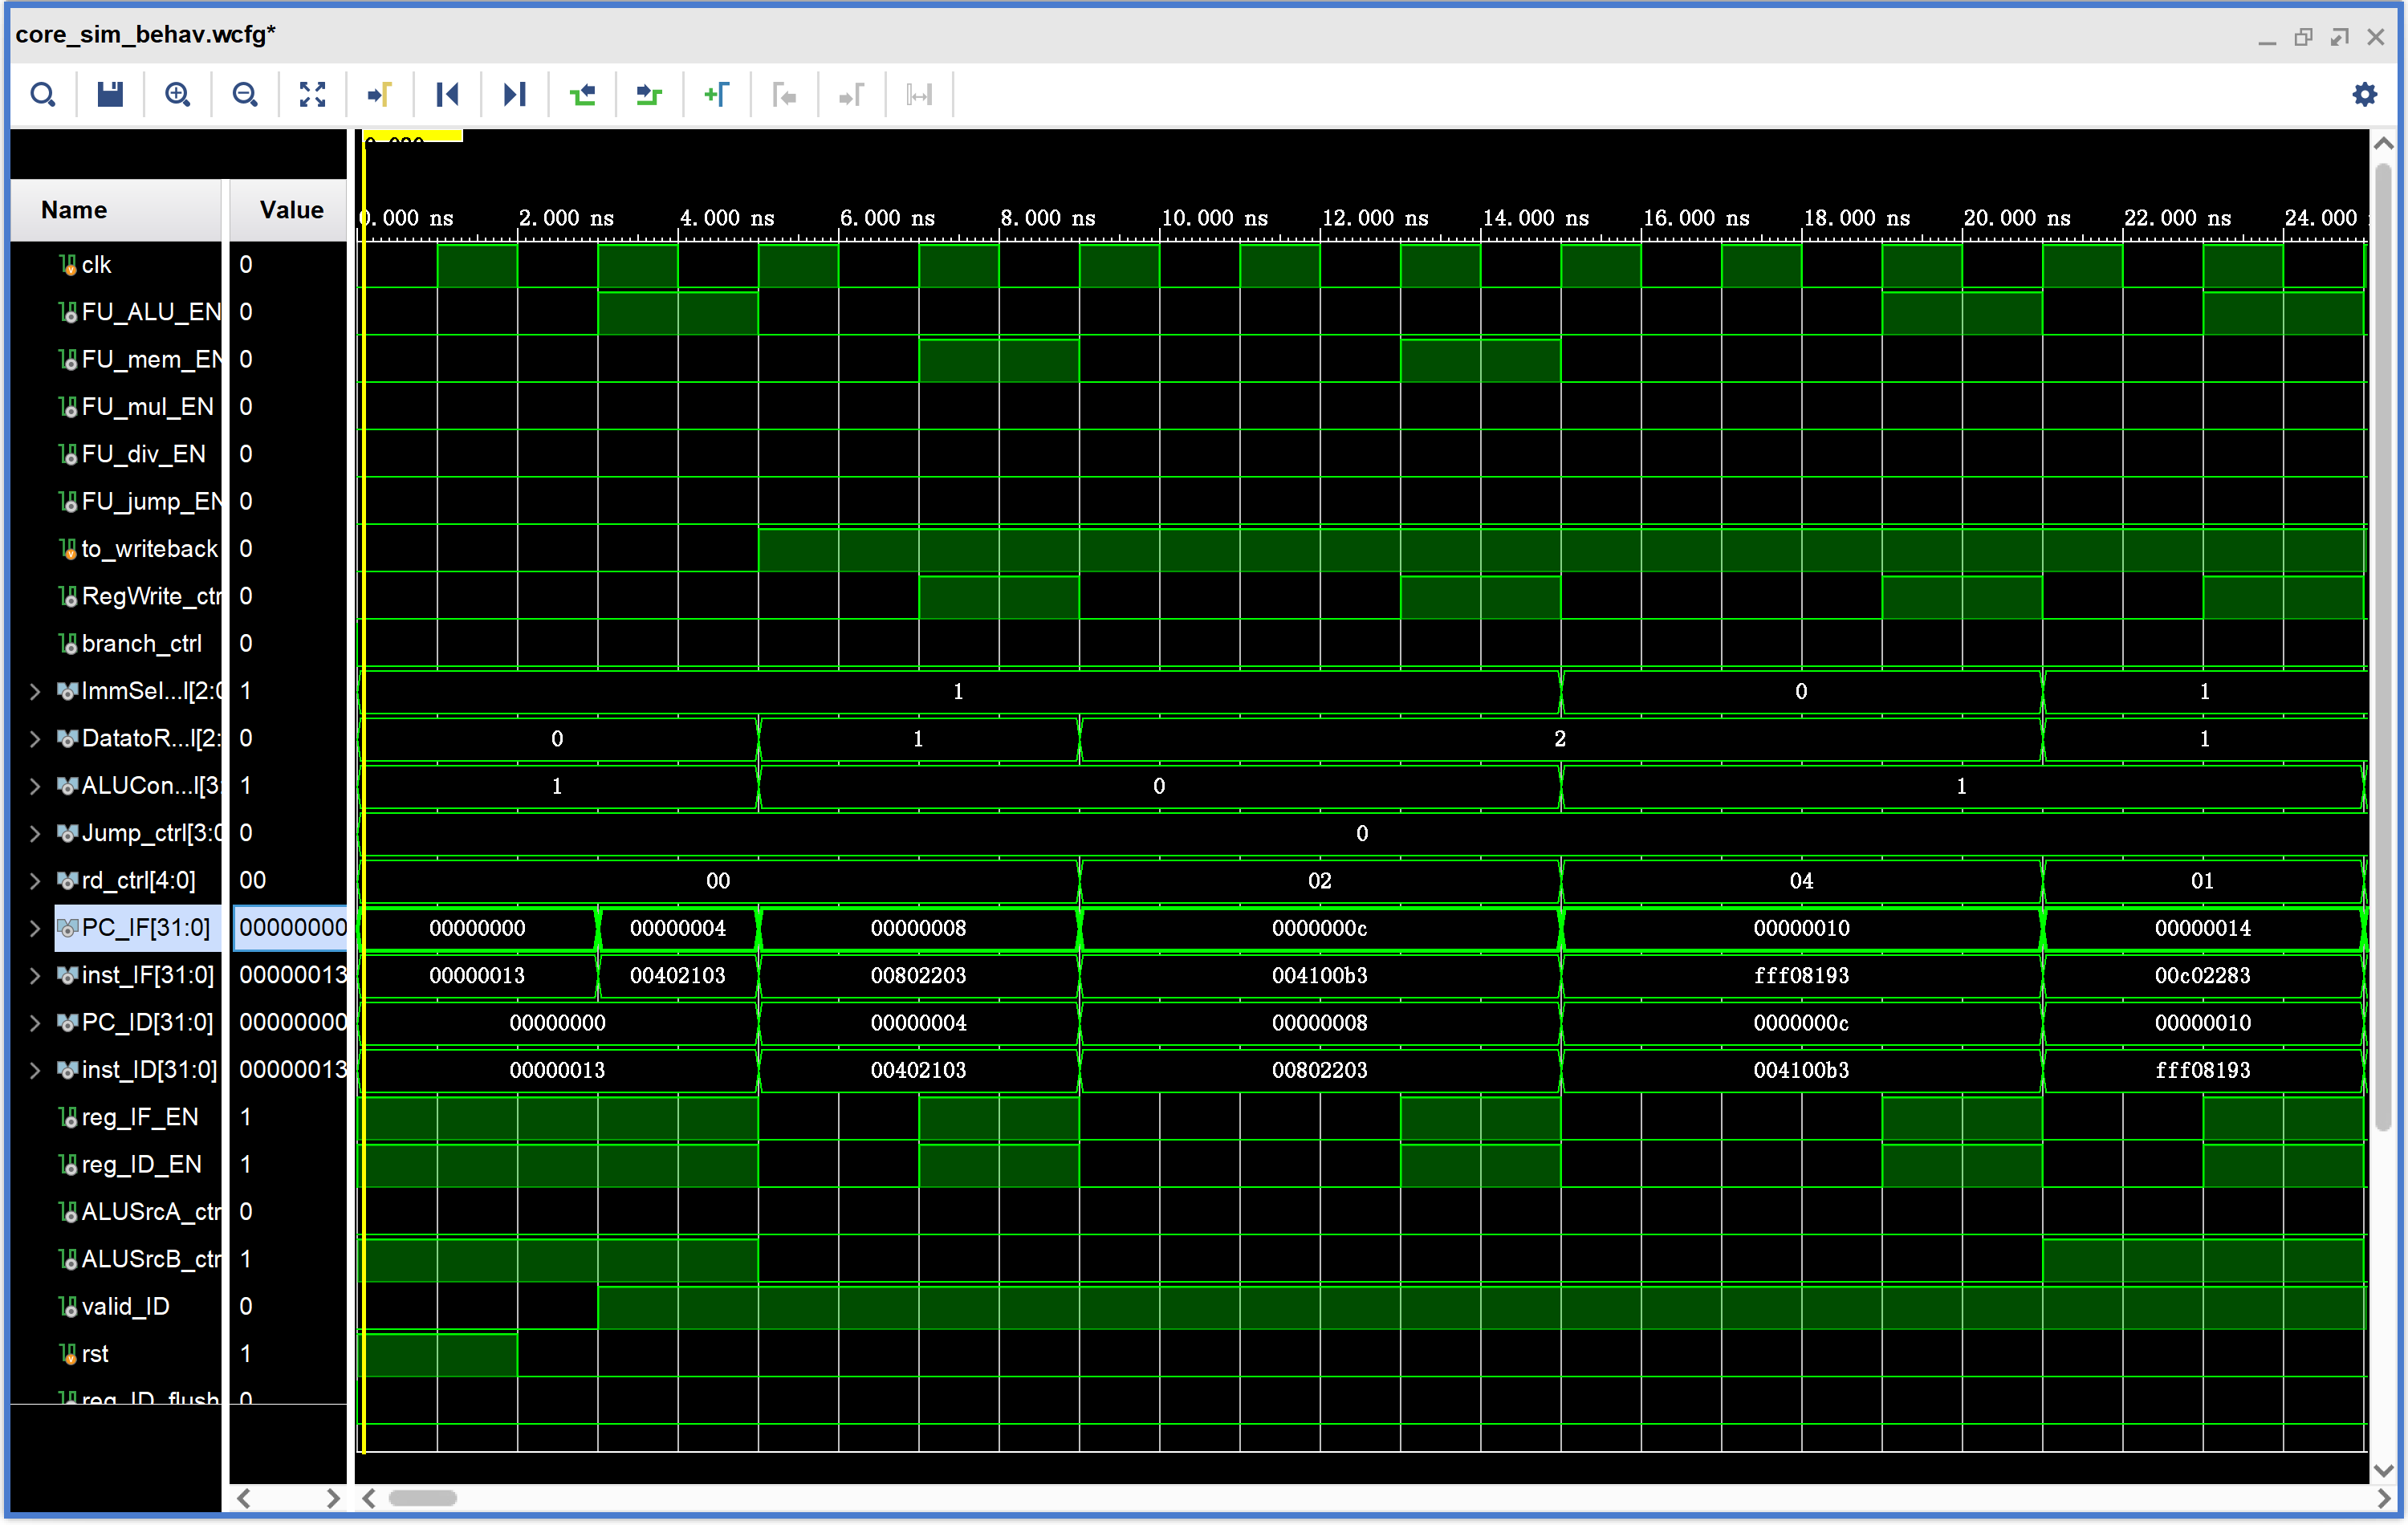
\includegraphics[width=1.0\textwidth]{figs/1.png} %插入图片,[]中设置图片大小,{}中是图片文件名
	\caption{load} %最终文档中希望显示的图片标题
	\label{Fig.4} %用于文内引用的标签
\end{figure}
load操作之后的ALU操作,由于需要用到之前的数据,发生了数据冒险。因此需要等待之前的指令完成之后才能执行。

\begin{figure}[H]
    \centering
    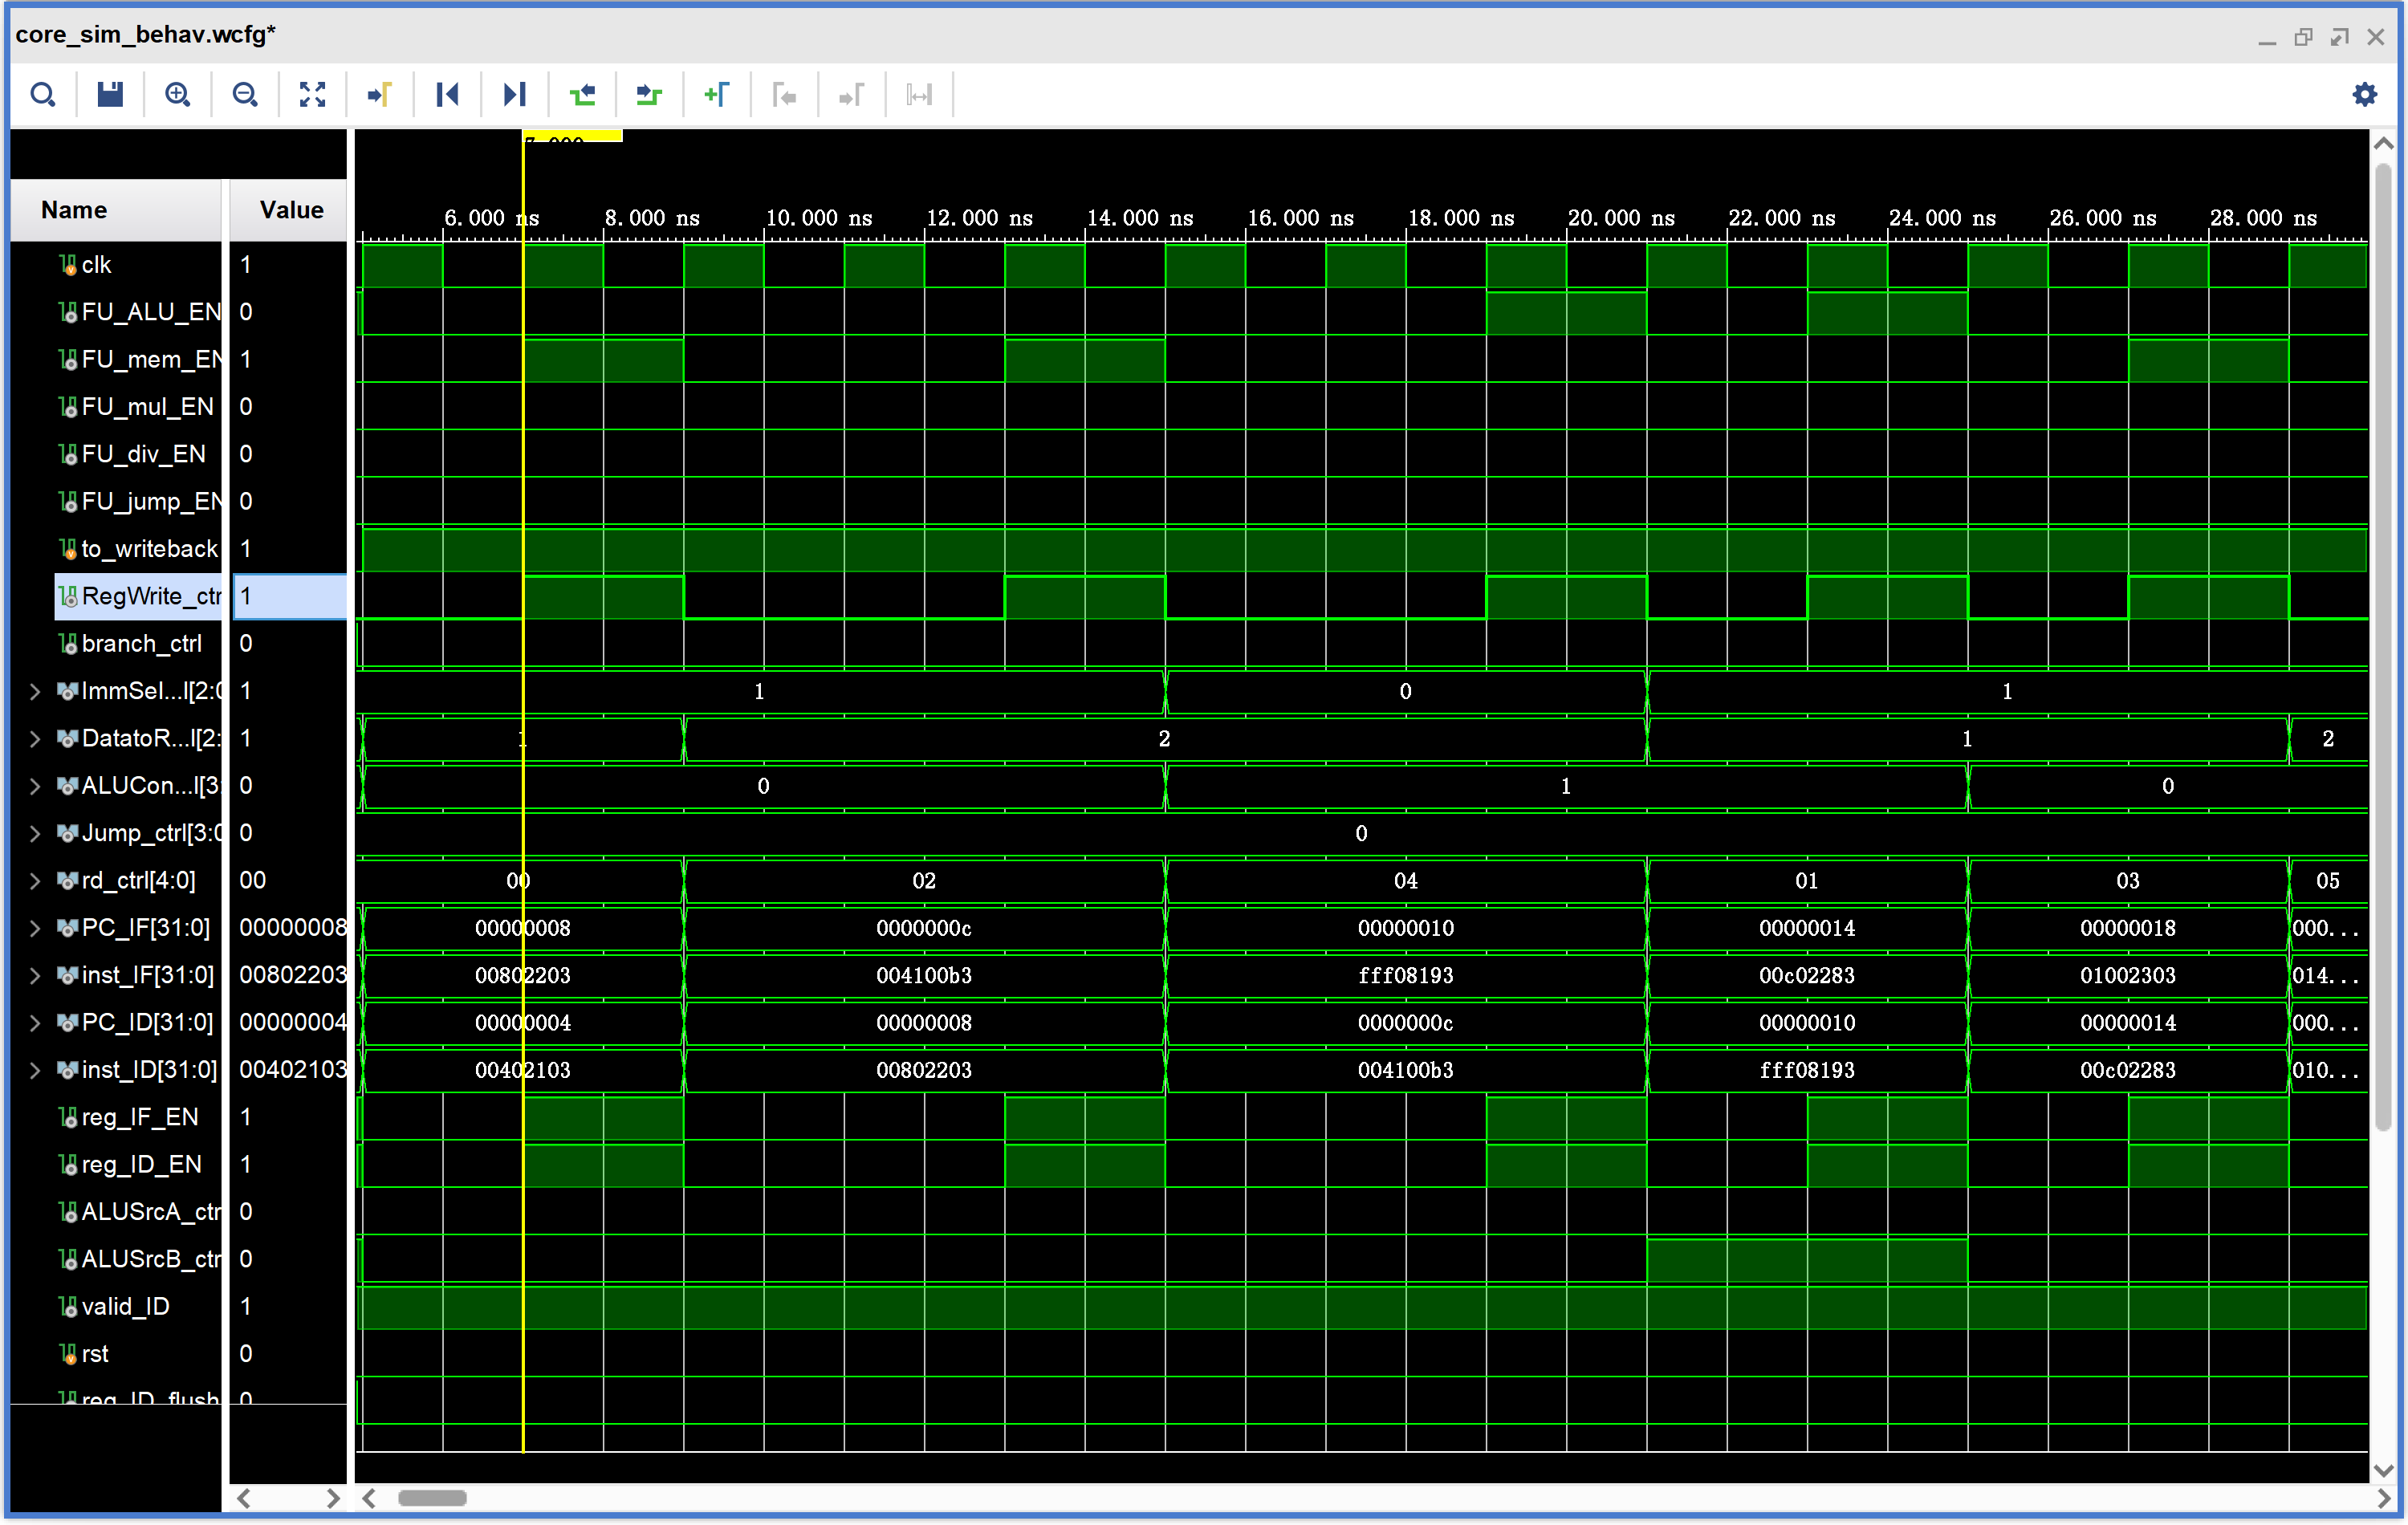
\includegraphics[width=1.0\textwidth]{figs/2.png}
    \caption{ALU}
    \label{Fig.5}
\end{figure}

在遇到branch指令时,采用predict not taken的方式。首先让程序继续执行,若发现需要进行跳转,则杀死branch指令之后的指令,并跳转至下一条指令的位置。

\begin{figure}[H]
    \centering
    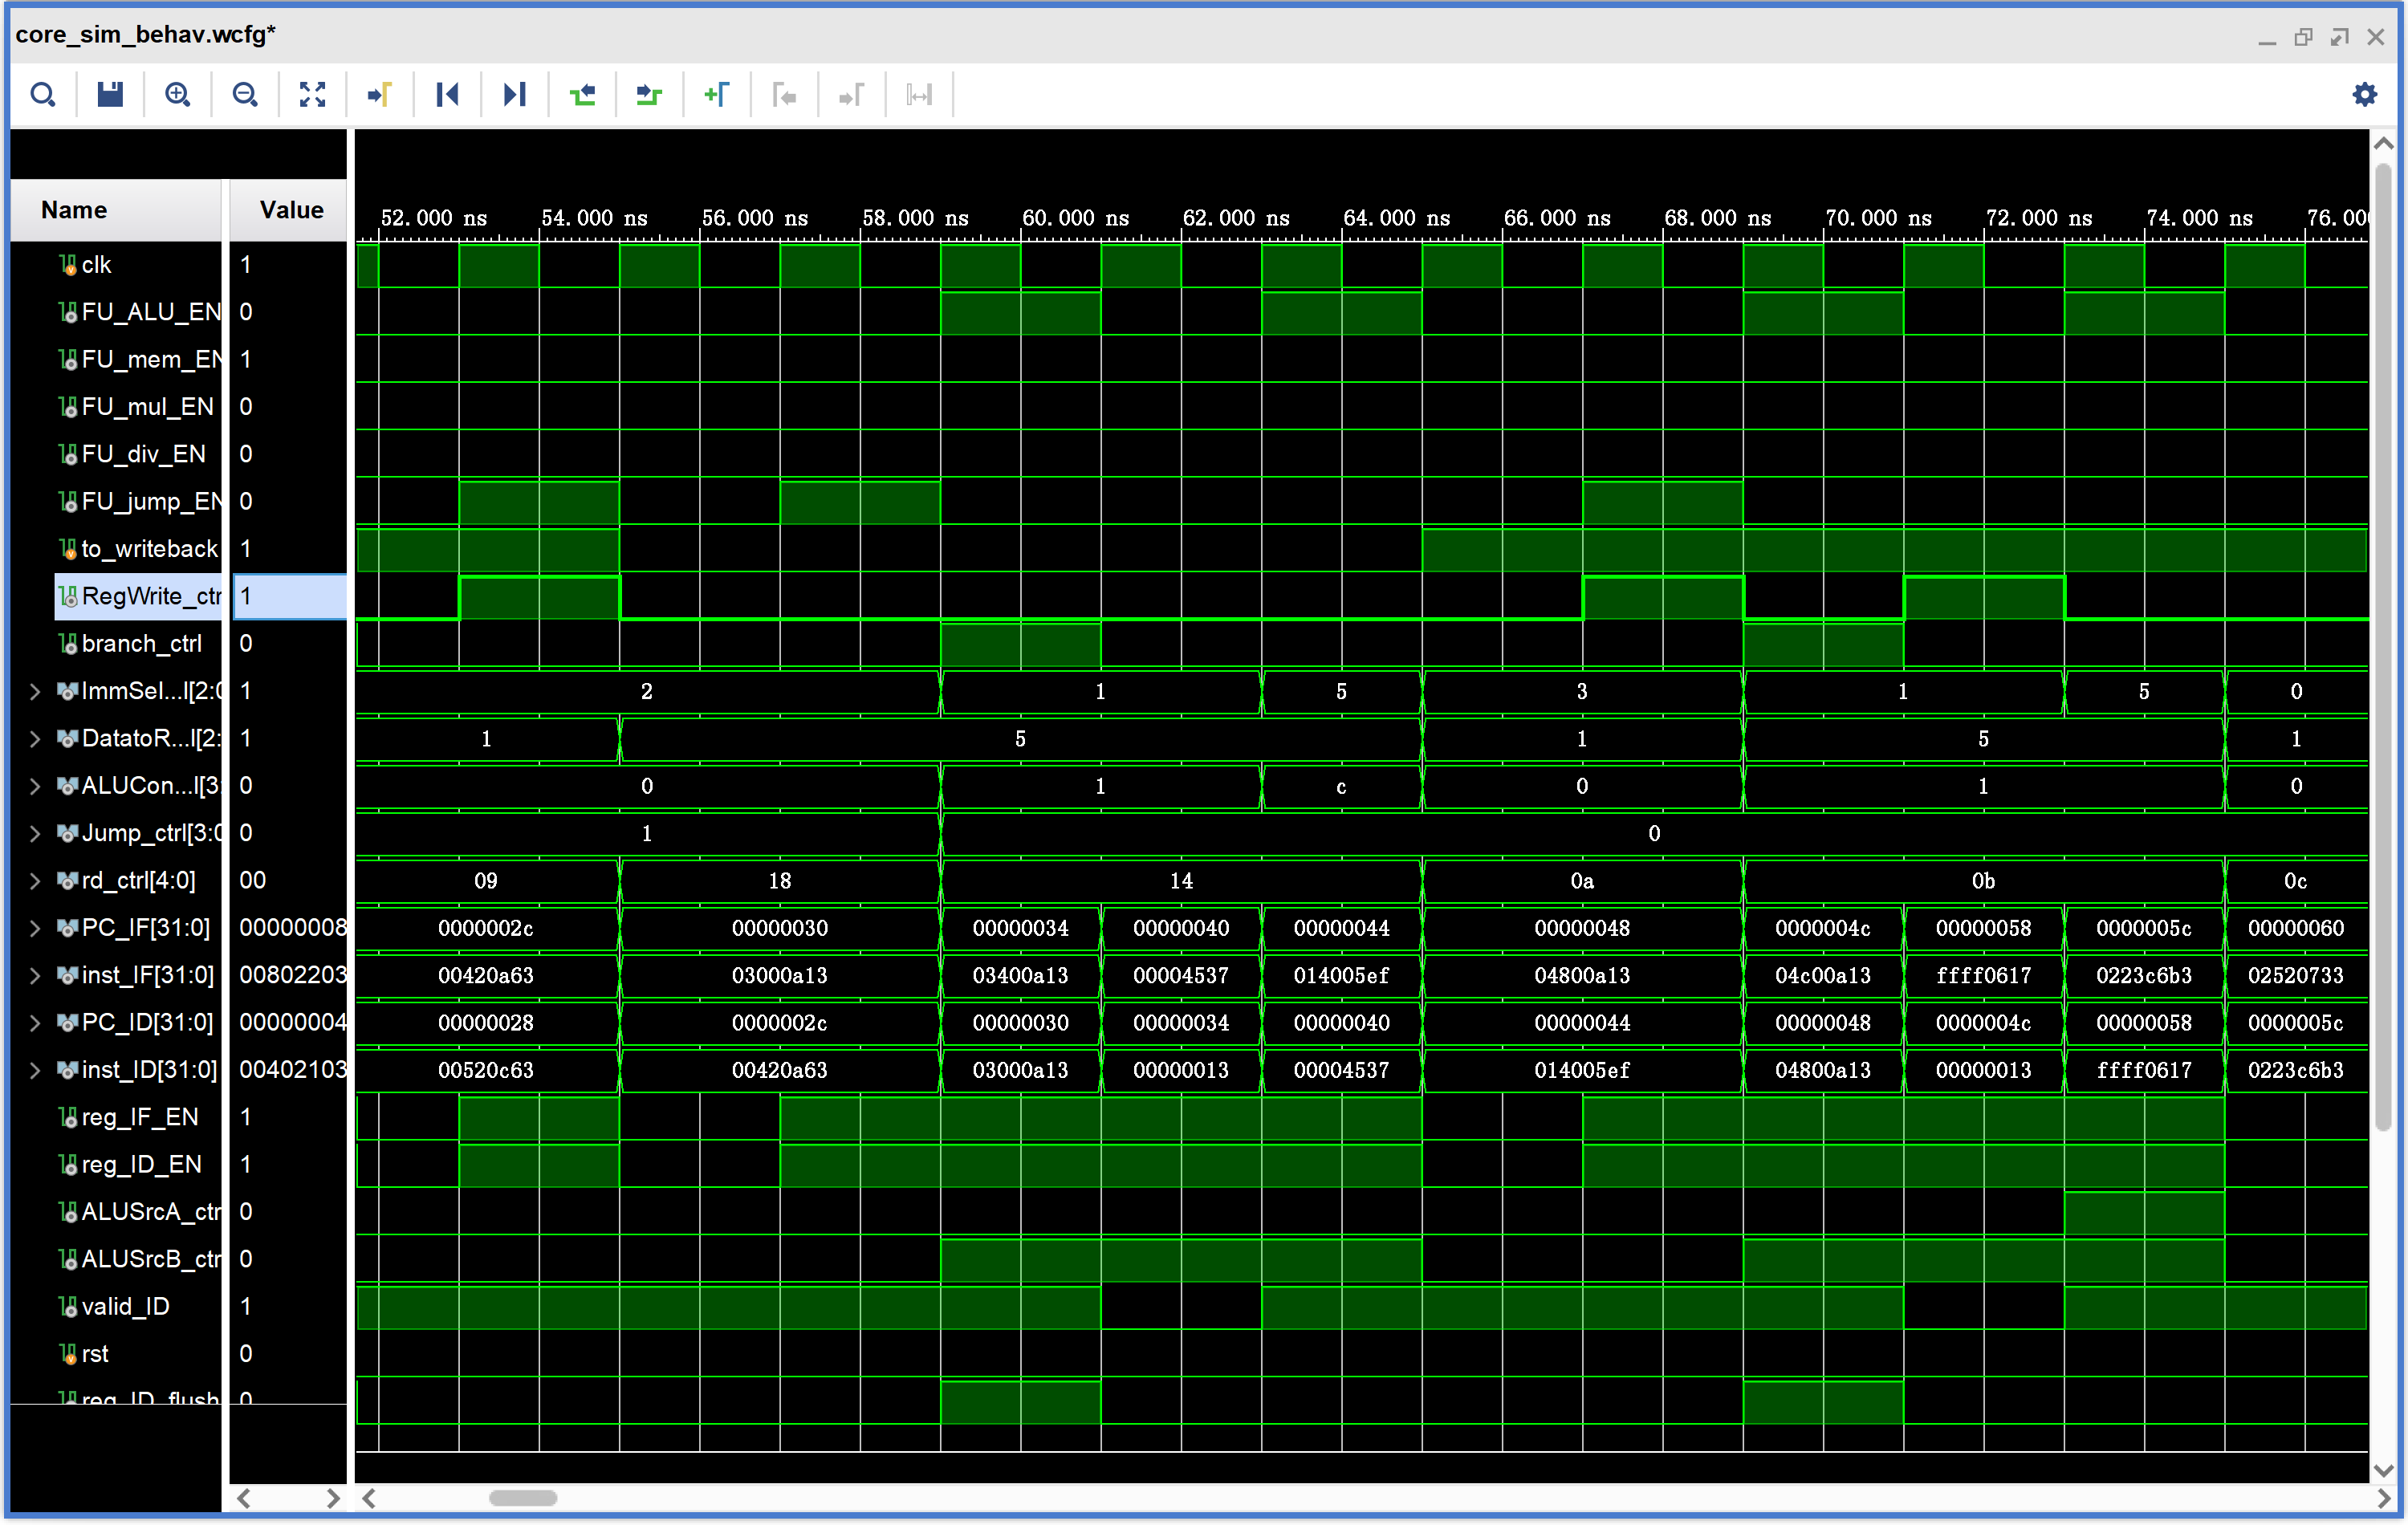
\includegraphics[width=1.0\textwidth]{figs/3.png}
    \caption{branch}
    \label{Fig.6}
\end{figure}

在遇到jal指令时,采取同样的操作

\begin{figure} [H]
    \centering
    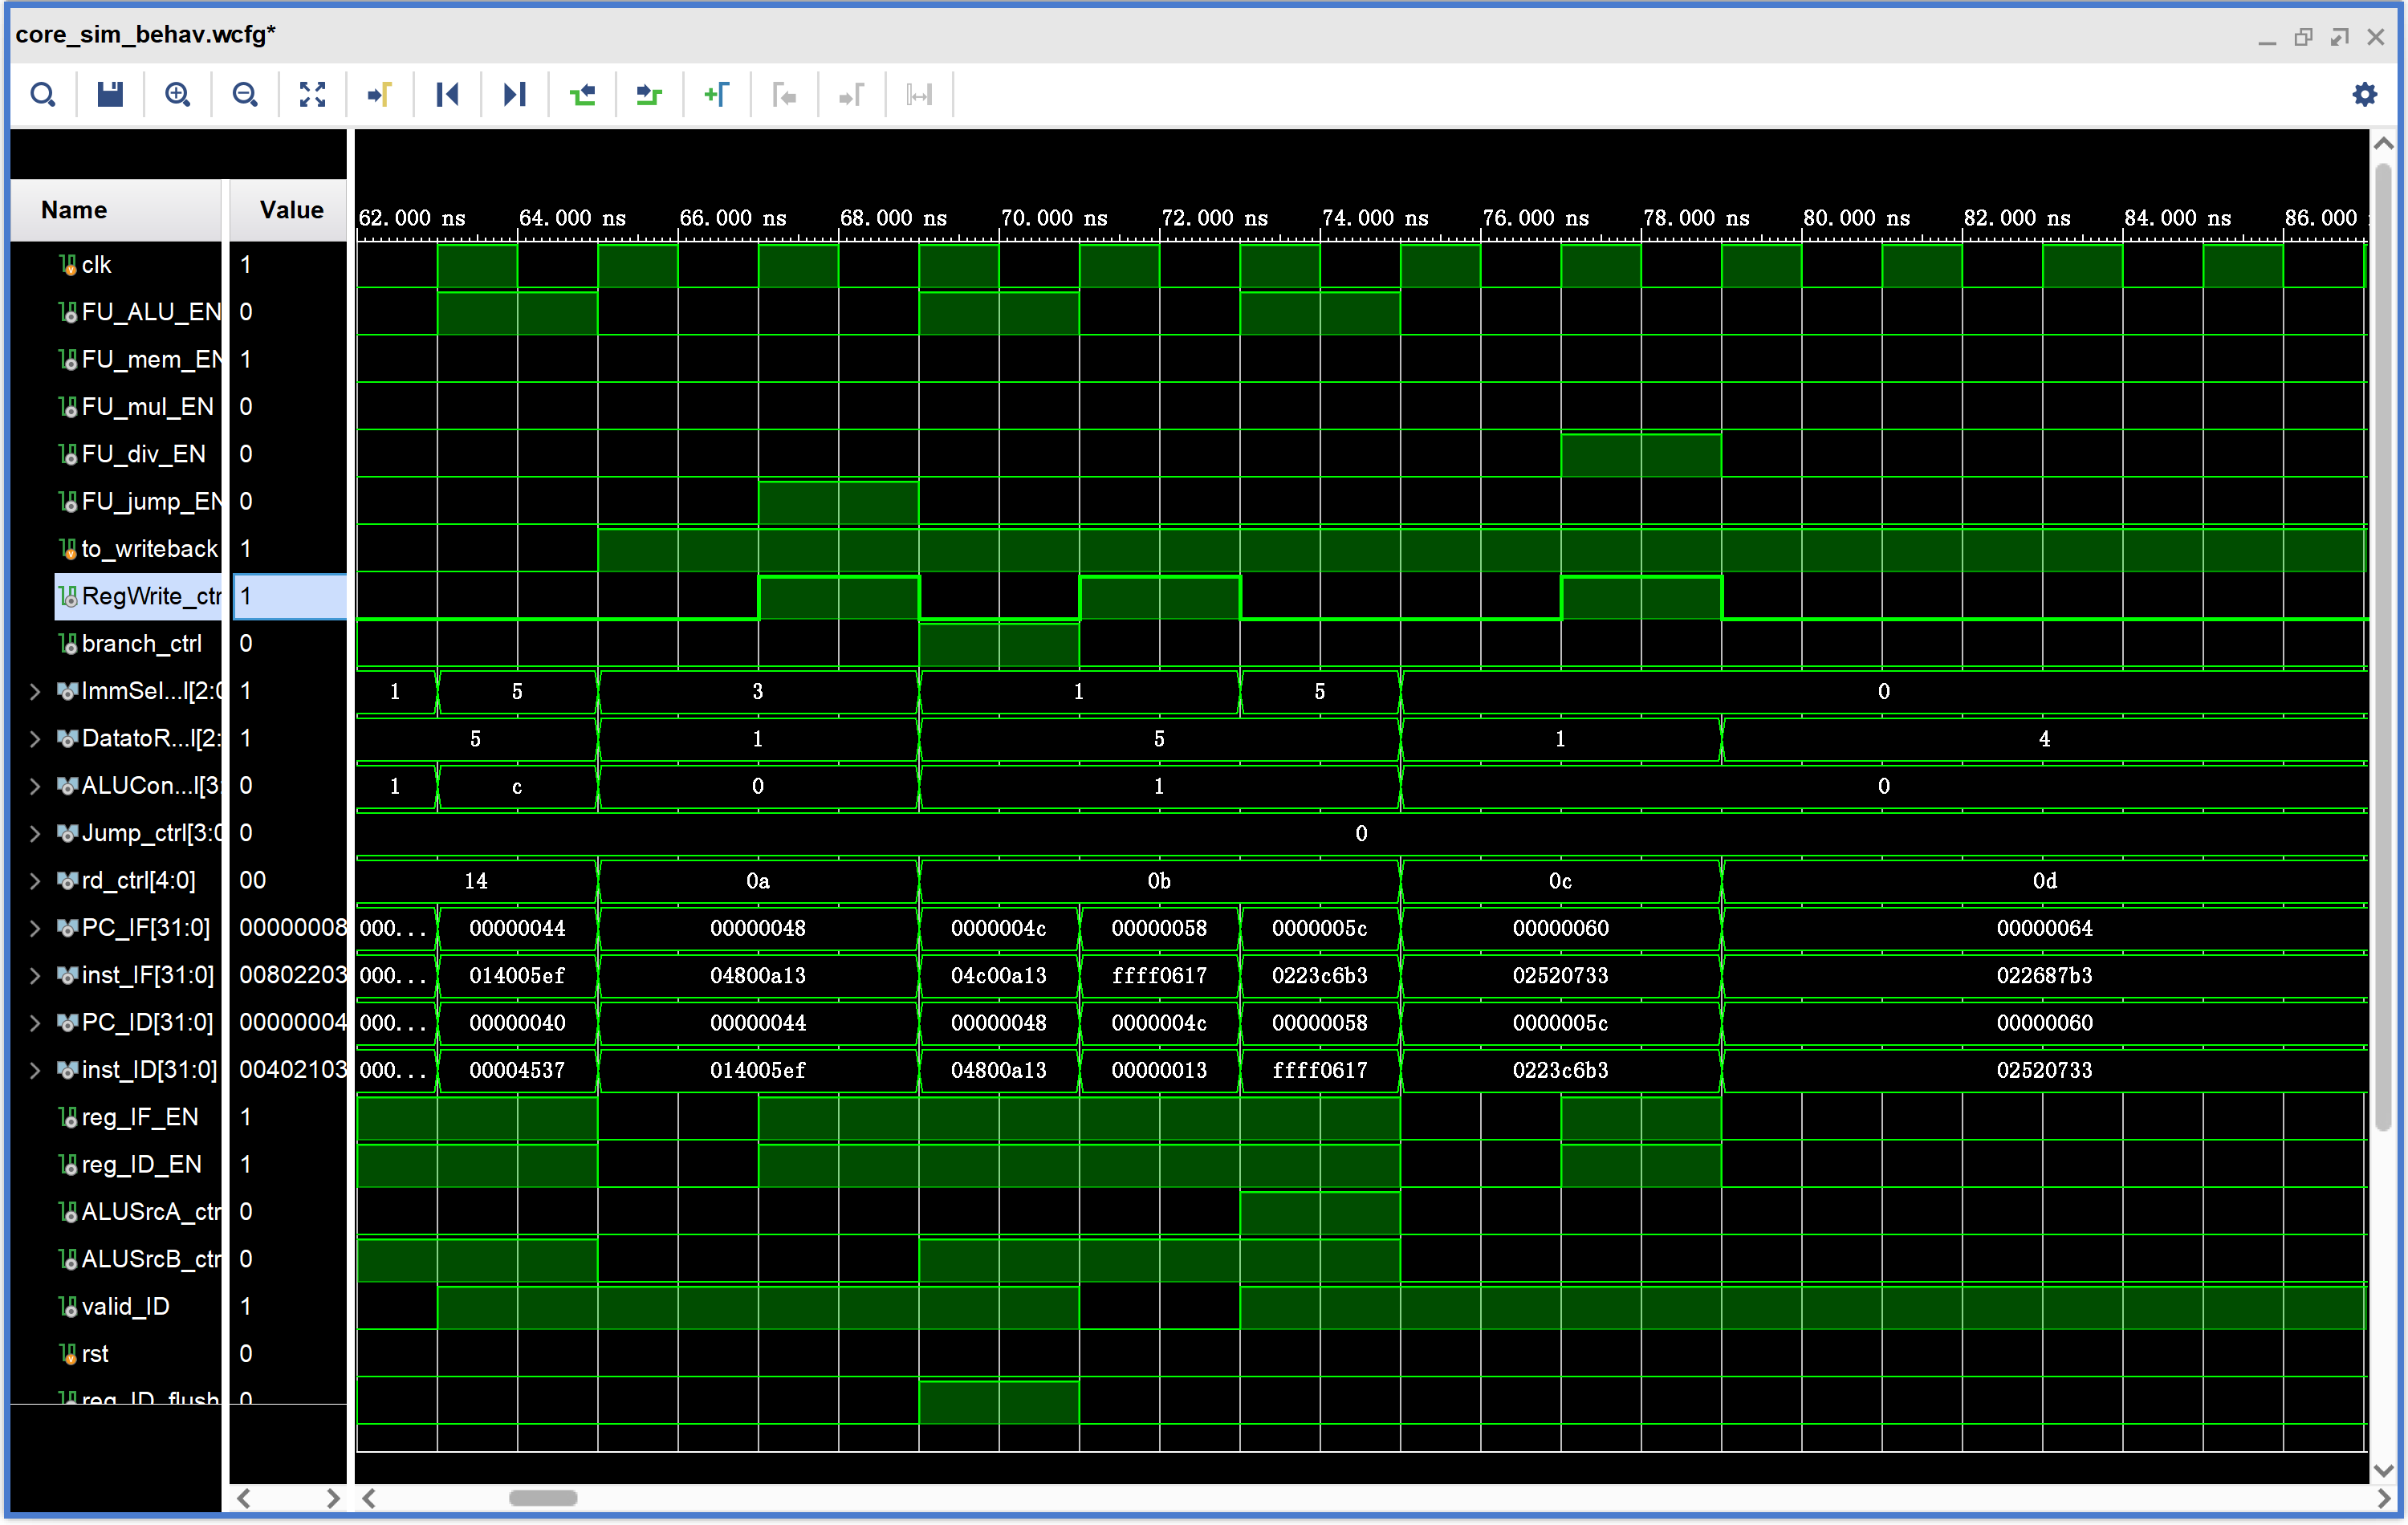
\includegraphics[width=1.0\textwidth]{figs/4.png}
    \caption{jal}
    \label{Fig.8}
\end{figure}

之后进入除法指令,一次除法需要很长的时间,具体实现由IP核提供

\begin{figure}[H]
    \centering
    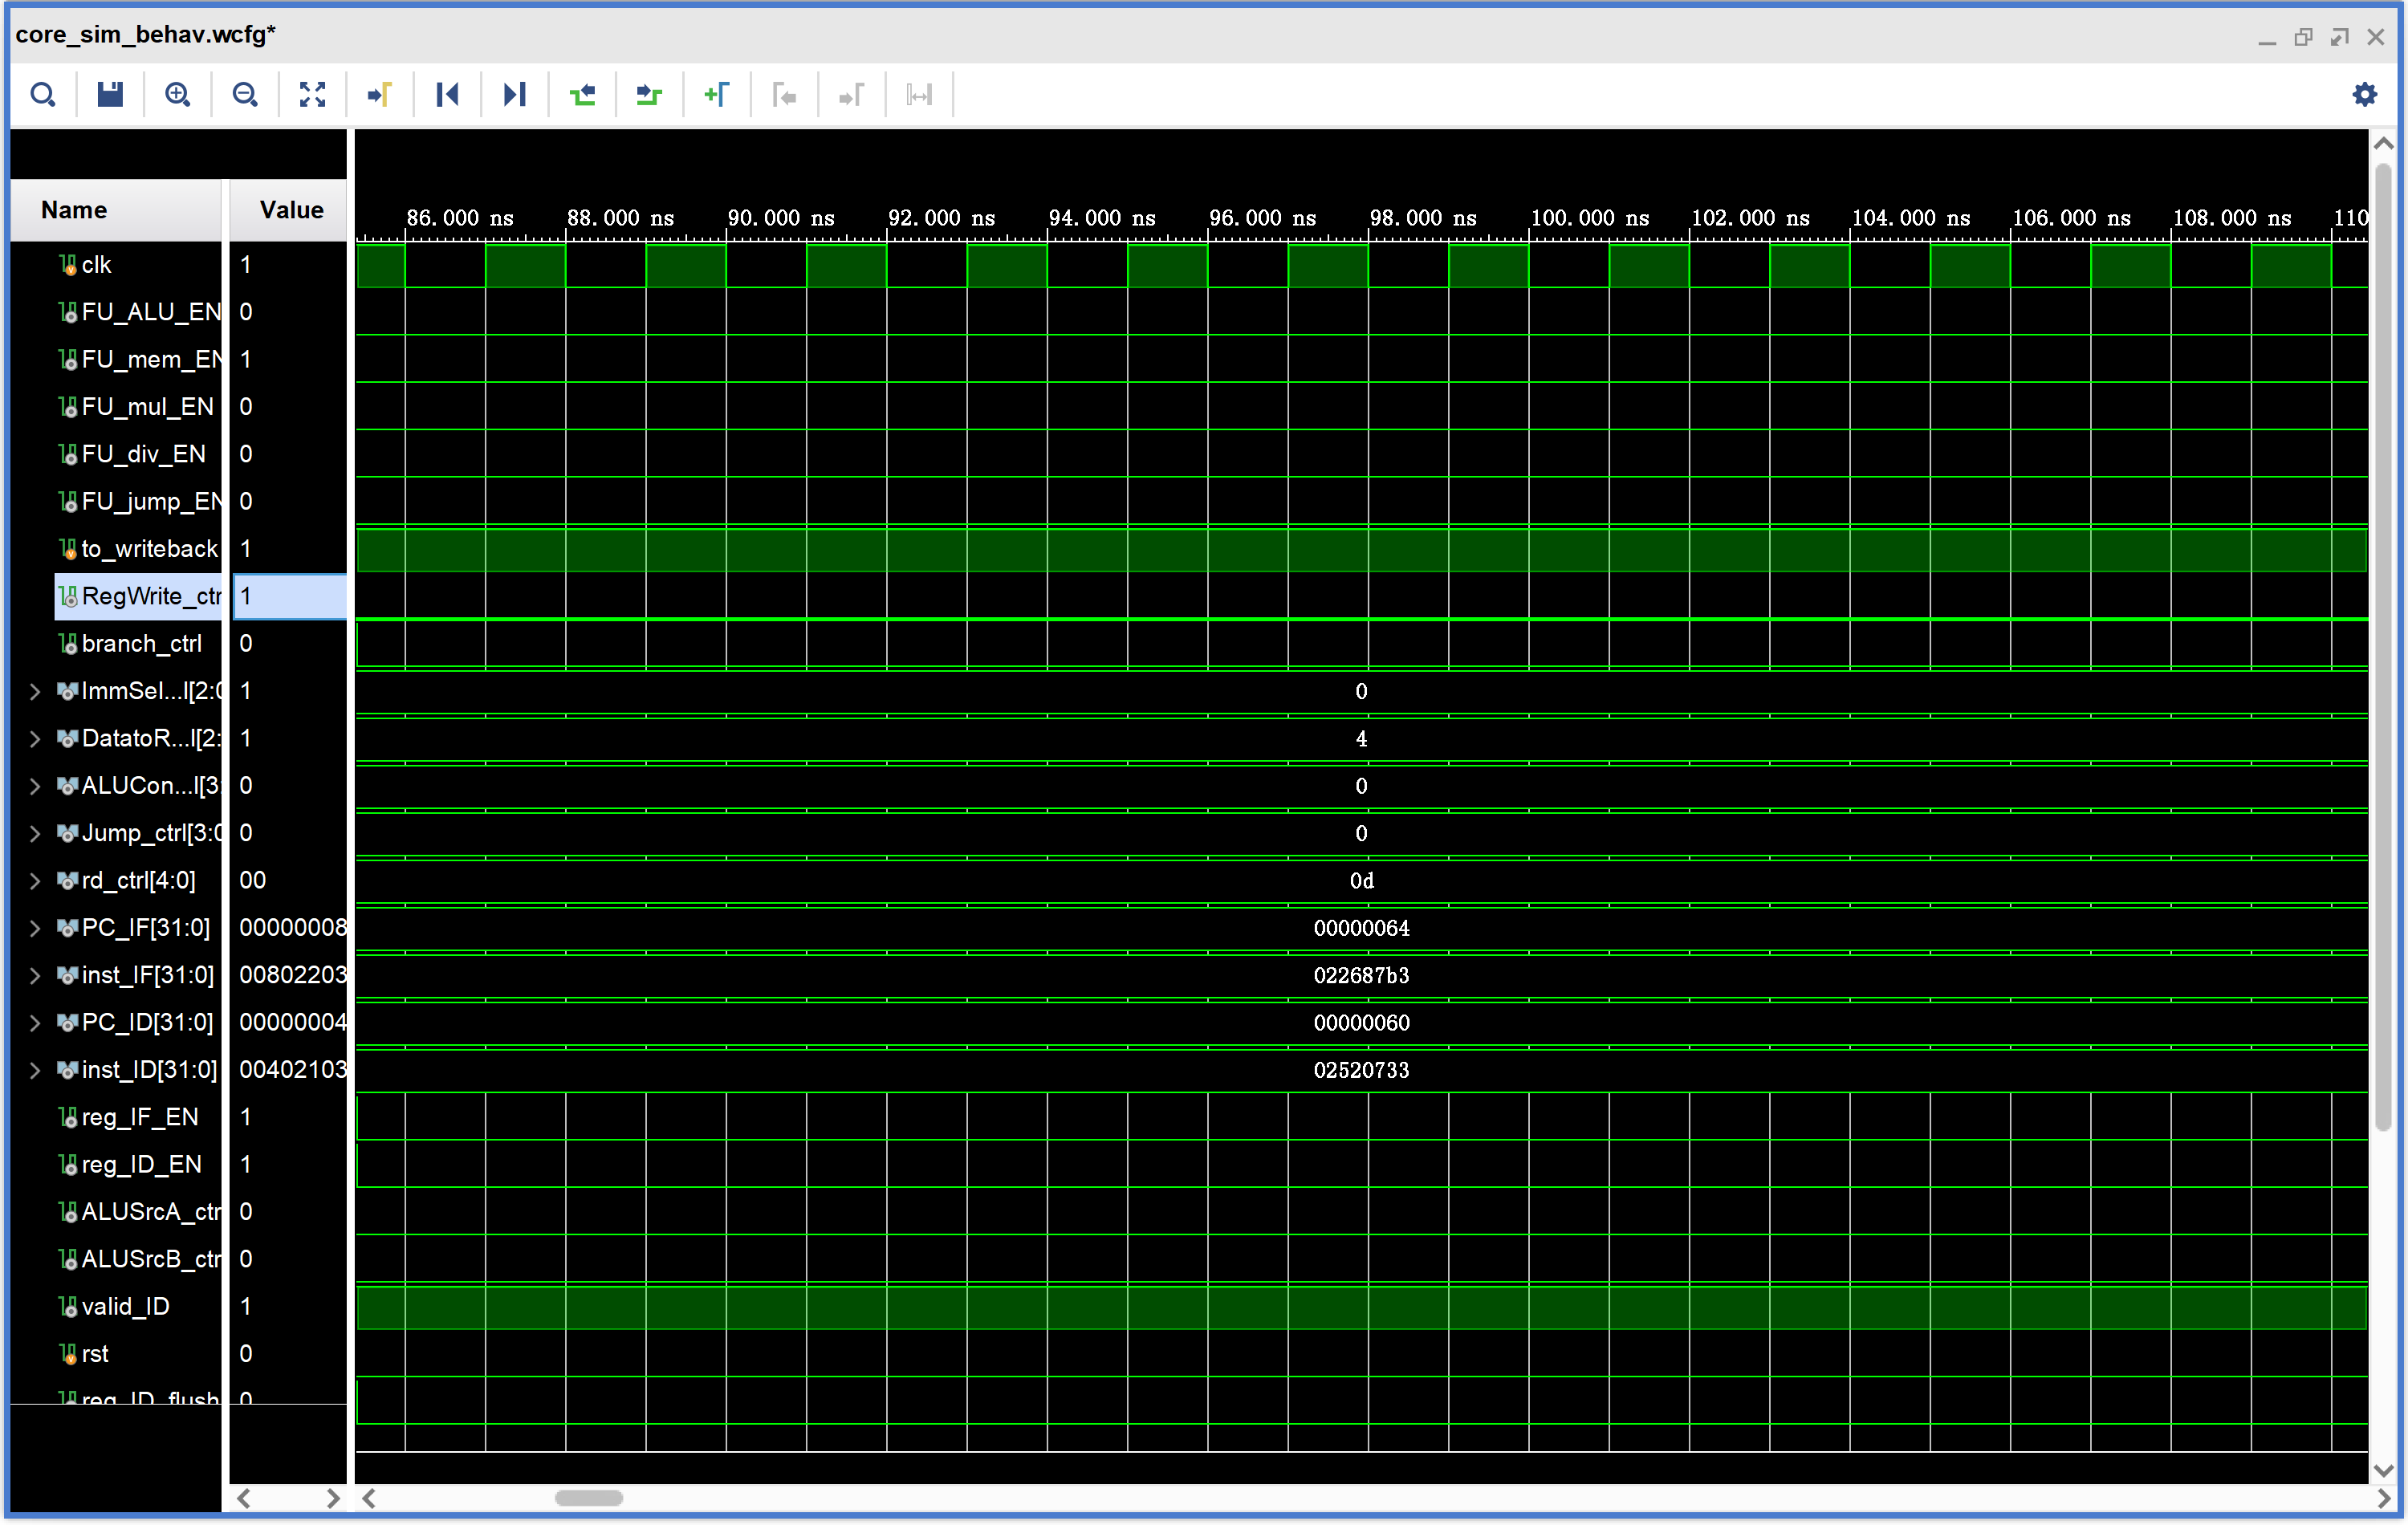
\includegraphics[width=1.0\textwidth]{figs/6.png}
    \caption{div}
    \label{Fig.9}
\end{figure}

后面是两条乘法指令,每条乘法指令的FU阶段需要多个周期

\begin{figure}[H]
    \centering
    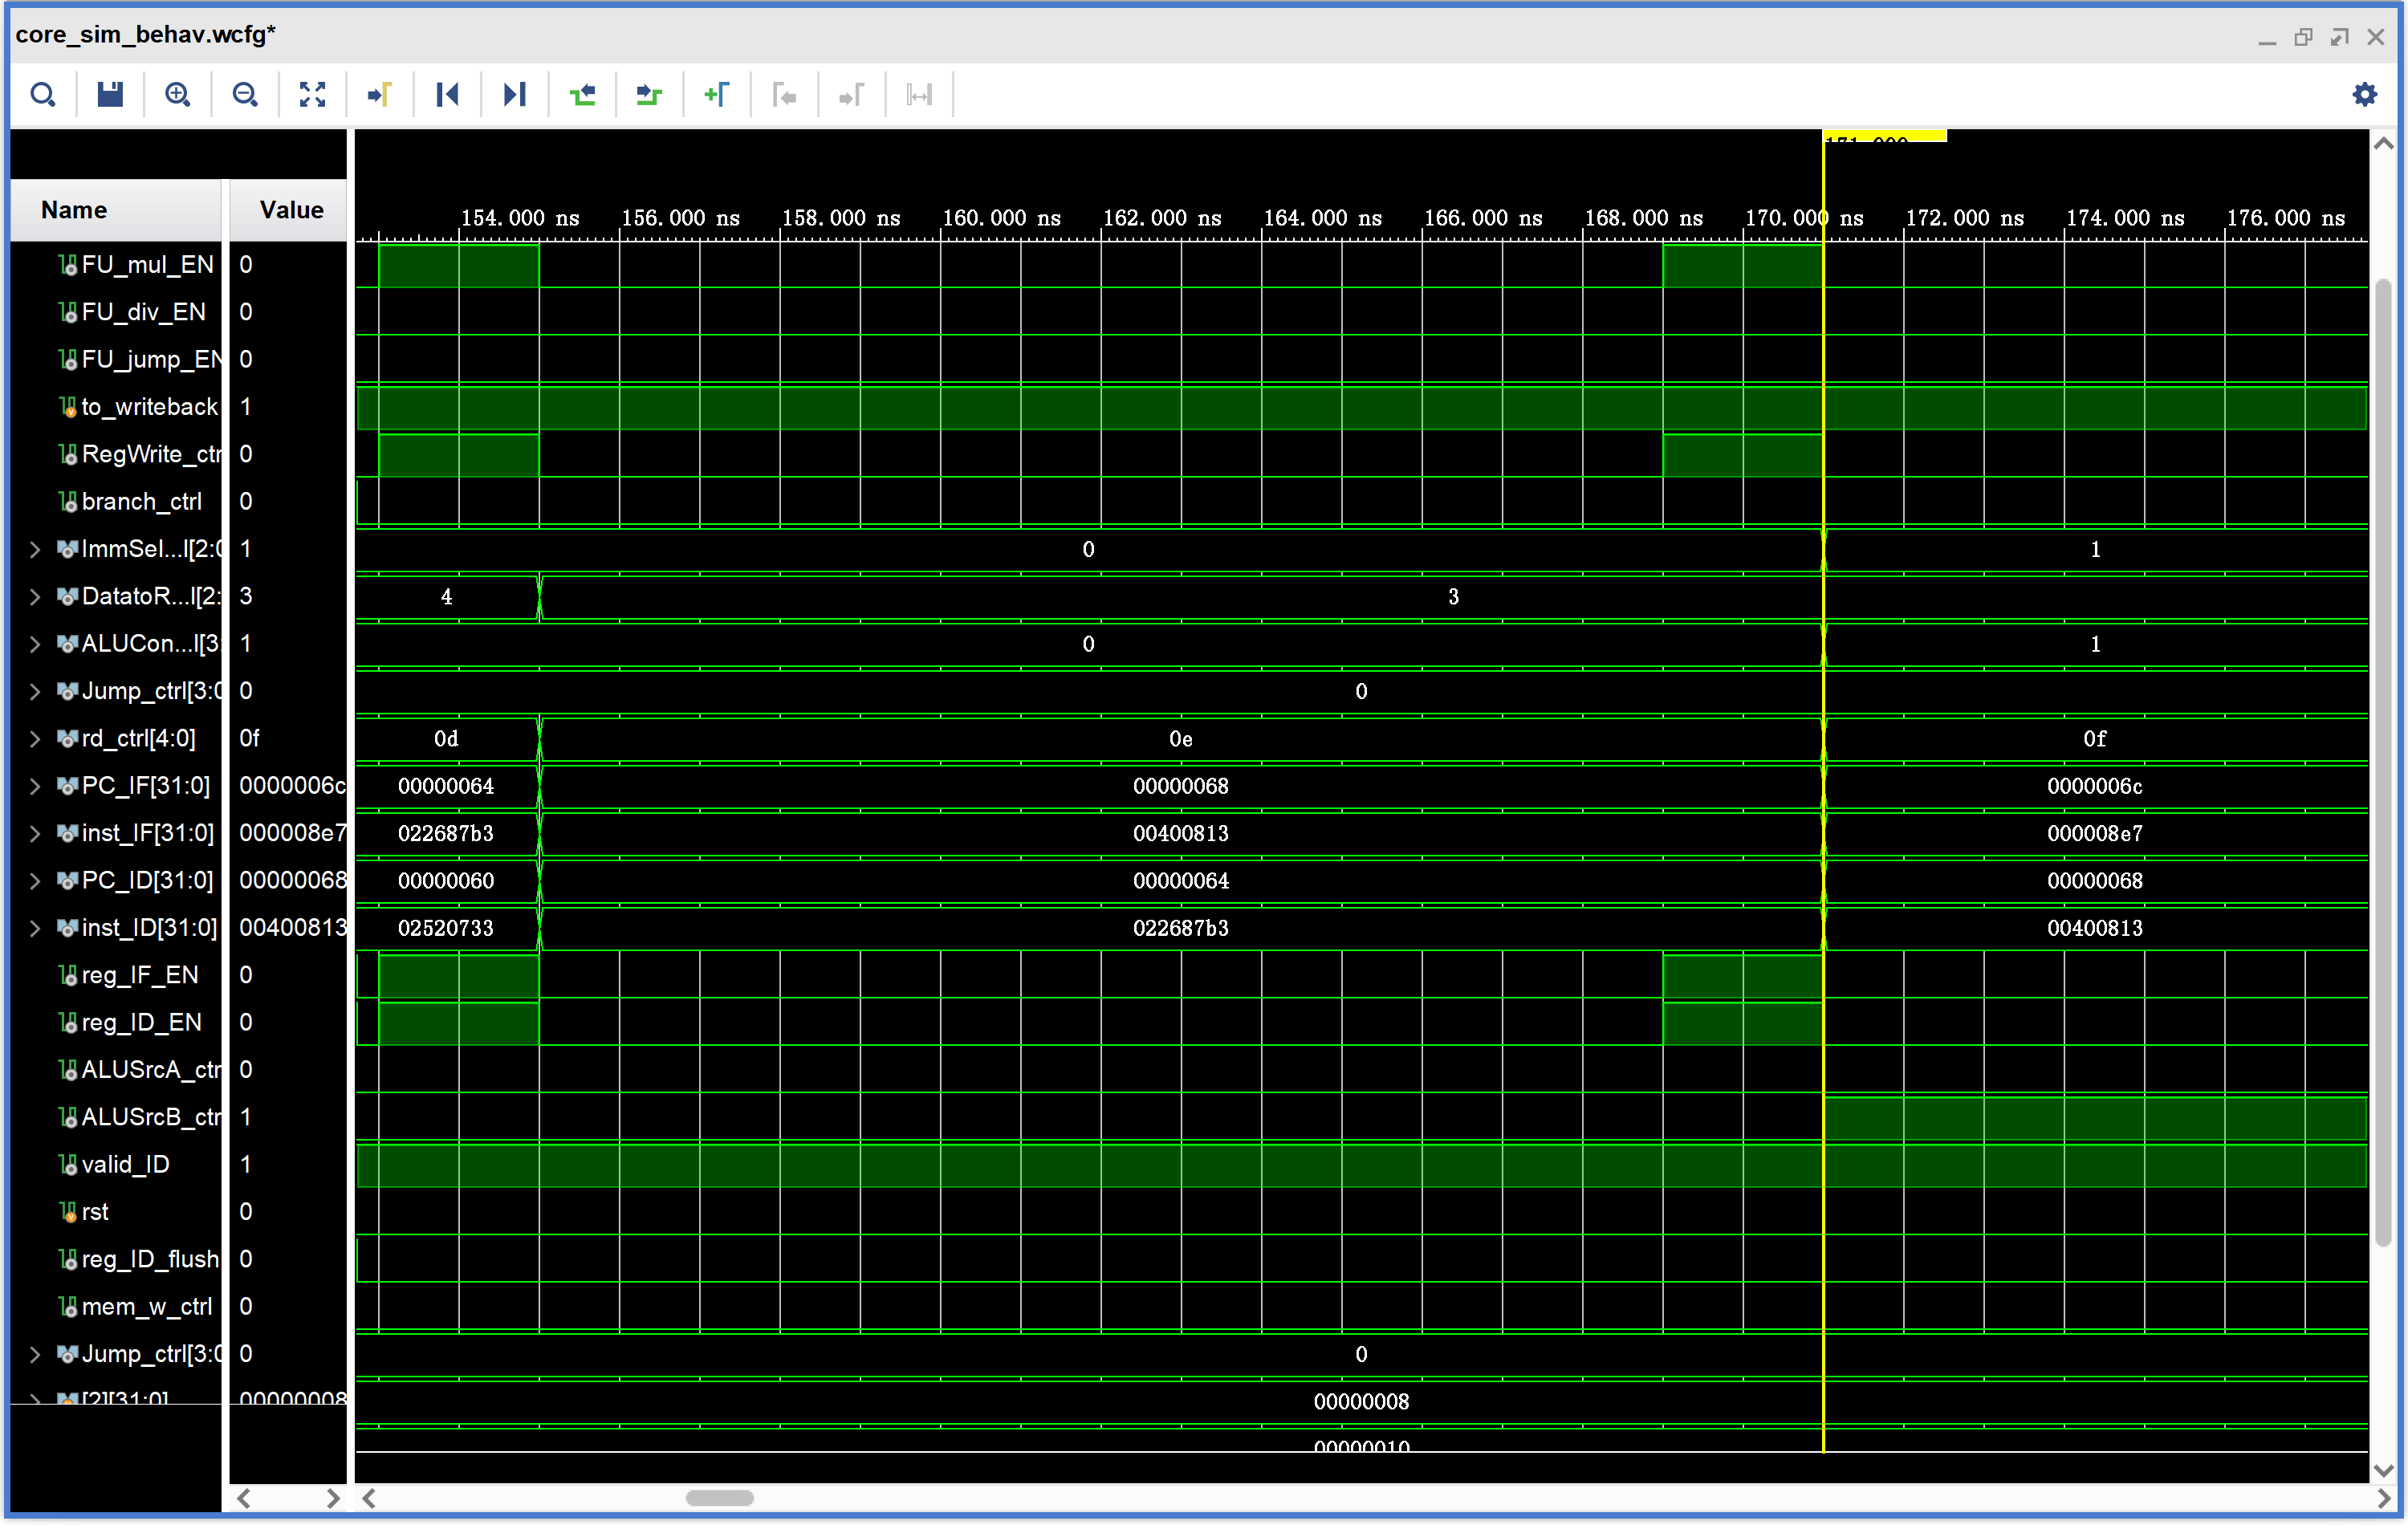
\includegraphics[width=1.0\textwidth]{figs/7.png}
    \caption{mul1}
    \label{Fig.10}
\end{figure}

\begin{figure}[H]
	\centering
	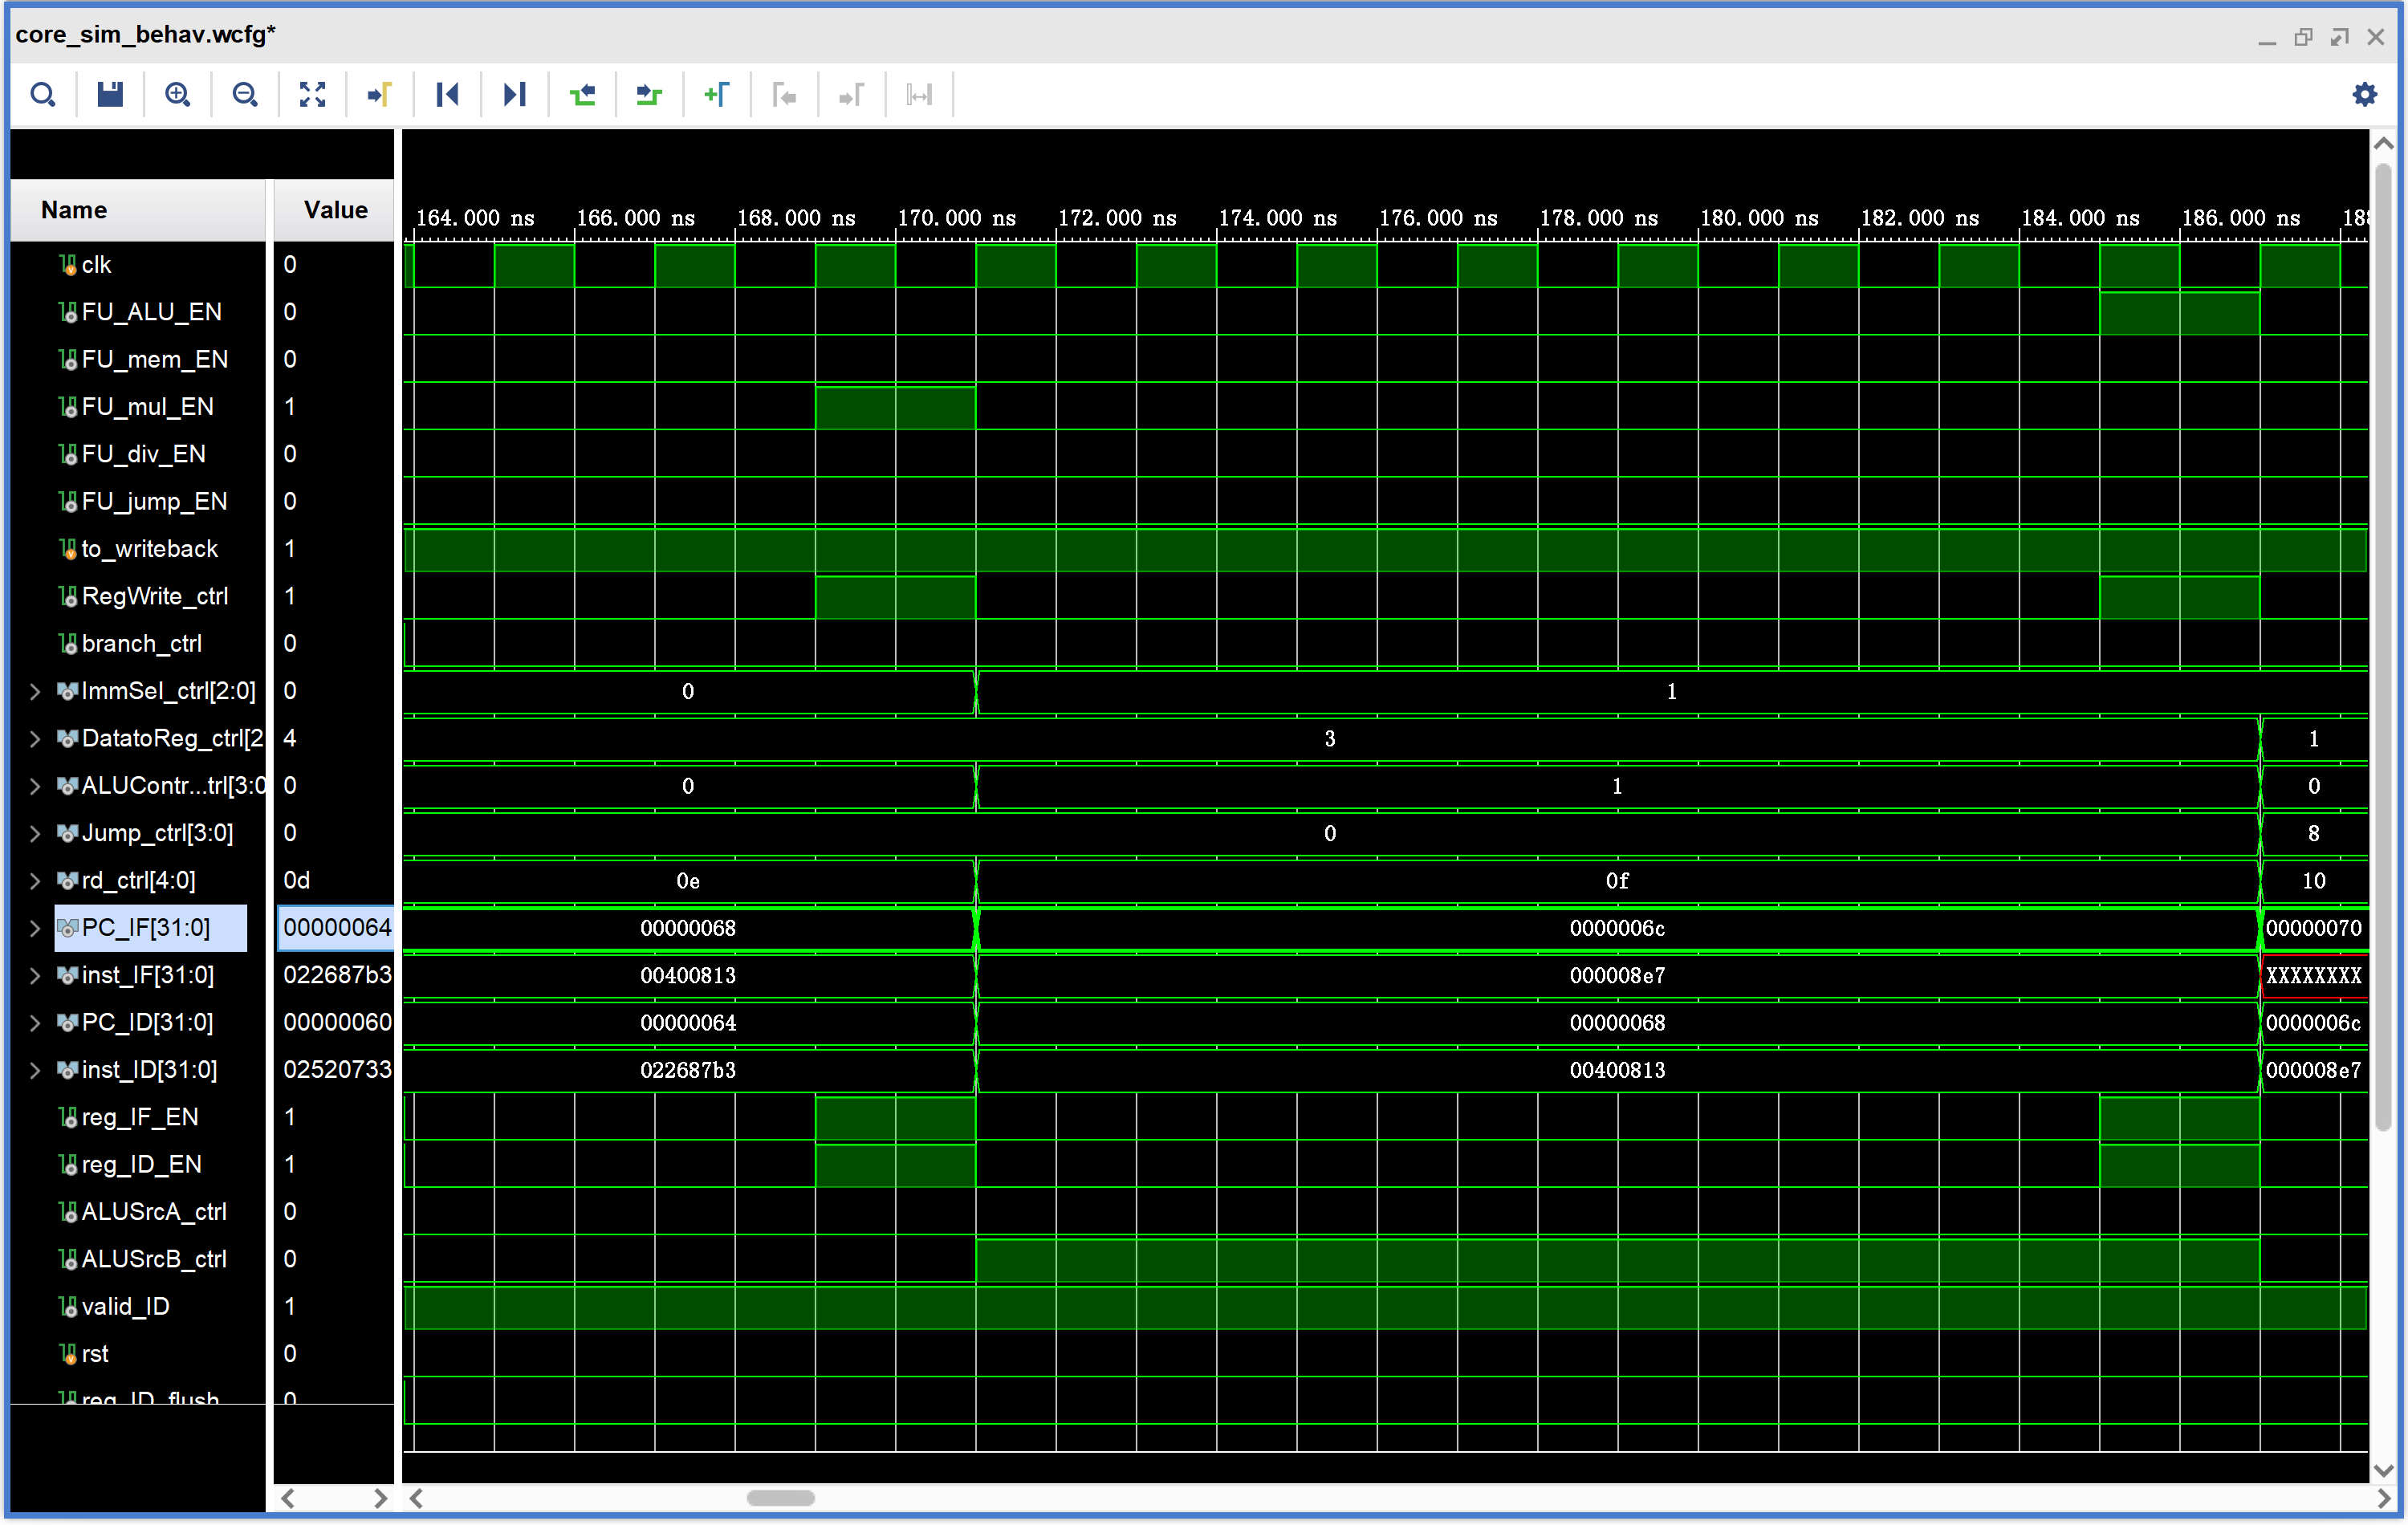
\includegraphics[width=1.0\textwidth]{figs/9.png}
	\caption{mul2}
	\label{Fig.12}
\end{figure}

最后,jalr指令使PC回到程序开头,进行下一次运行。
由于在跳转回去之前,CPU会读取jalr之后的指令,但jalr之后没有新的指令,因此读取会出现错误,会出现大片红色。

\begin{figure}[H]
    \centering
    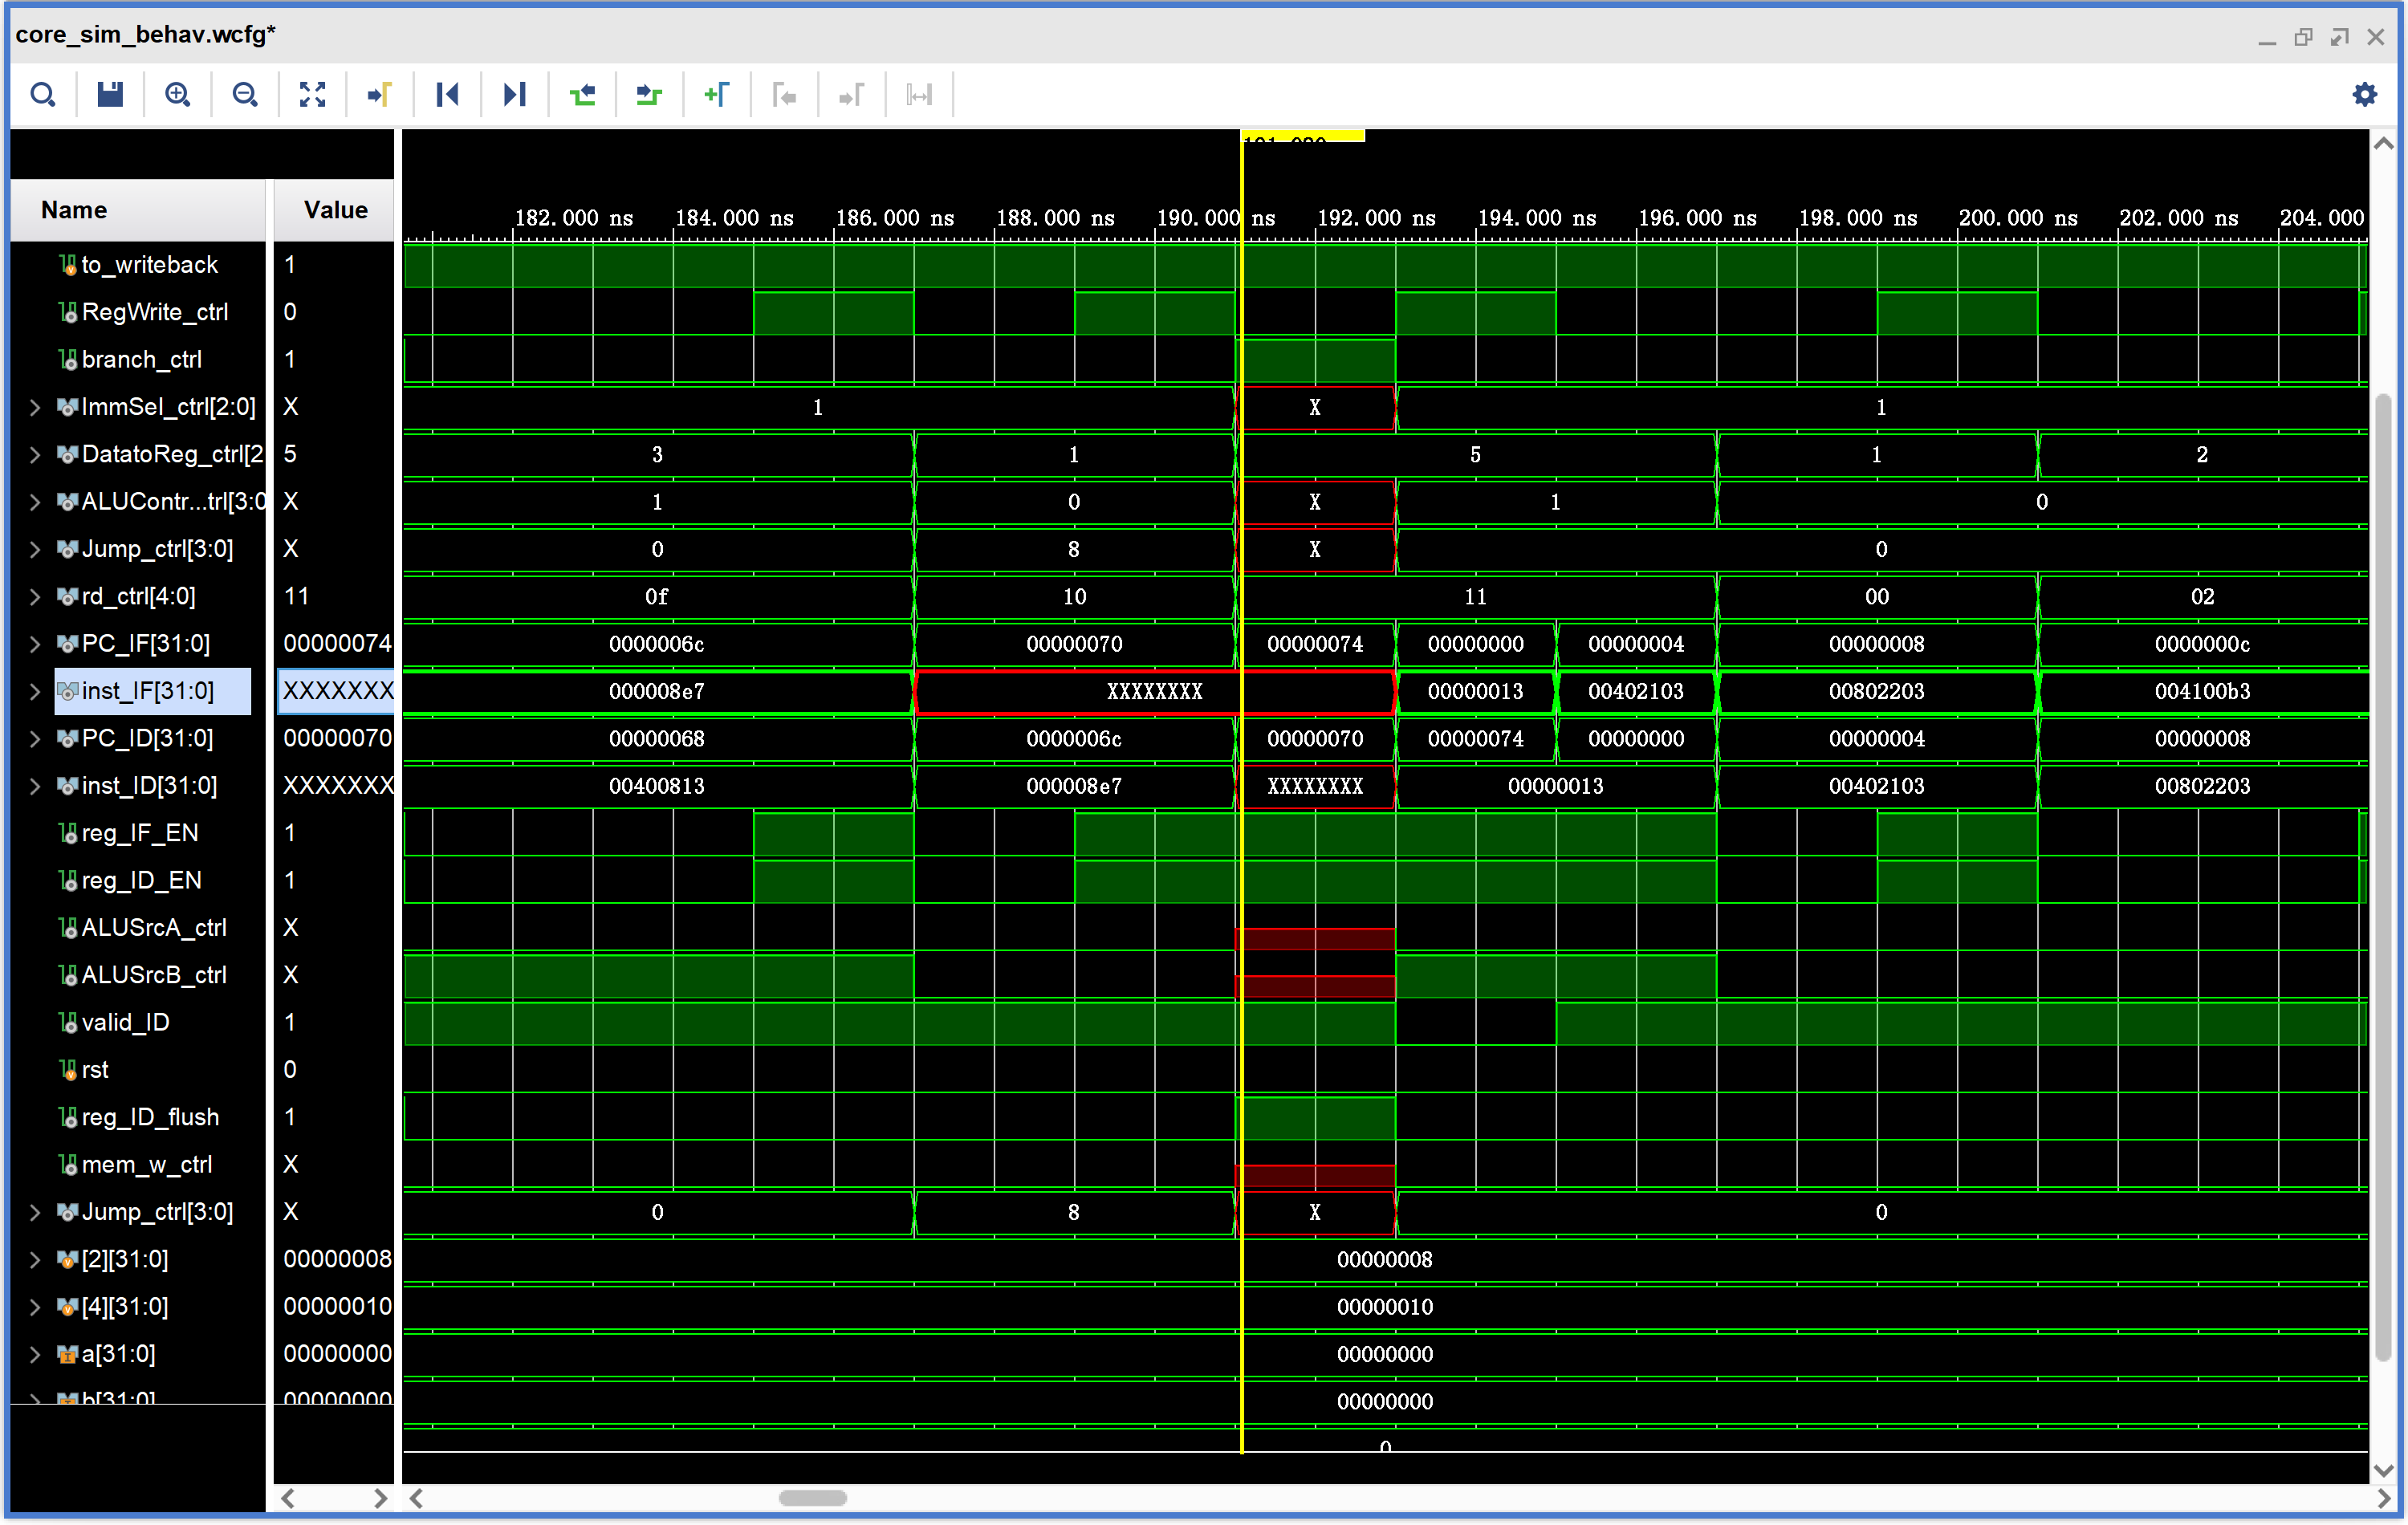
\includegraphics[width=1.0\textwidth]{figs/8.png}
    \caption{jalr}
    \label{Fig.11}
\end{figure}

\subsection{上板结果分析}
仿真结果正确已经基本验证了实验的正确性,下面我组再简单的通过几张结果截图分析正确性。


后续的流程类似,均符合上部分仿真结果,具体流程会在验收时展示。